% !TeX spellcheck = ru_RU
% !TEX root=../main.tex

\begin{lecture}[Применение электродинамики к описанию растворов]
	Рассмотрим в этой лекции теорию Дебая-Хюккеля. Рассмотрение будем проводить на примере $ Na^+ Cl^- $. Введем характерную длину:
	\begin{equation}
	\lambda \sim \sqrt{\dfrac{l kT}{ne^2}}
	\label{eq:debay_lambda}
	\end{equation}
	Будем говорить о концентрации как о количестве частиц $ N $ в единице объема $ V $. ,,Садимся'' на $ Na $; все величины далее рассматриваются в среднем.
	
	\begin{center}\begin{tabular}{cc}
		$ \nabla^2 \varphi = - \dfrac{4 \pi \rho}{\varepsilon} $ & $ \rho = \rho (\vec{r}), ~~ \varphi = \varphi (\vec{r}) $ \\
		\multicolumn{2}{c}{$ \rho = n_1 \cdot Z_1 e + n_2 \cdot Z_2 e + \dots = \sum\limits_i n_i e Z_i $} \\
		\multicolumn{2}{c}{$ n_i = n_i^2 \cdot \underbrace{\exp\left[ - \dfrac{Z_i e \varphi}{kT} \right]}_{\text{Больцман}} $} \\
		\multicolumn{2}{c}{$ \Delta \varphi = -4 \left( \dfrac{\pi e}{\varepsilon} \right) \displaystyle \sum\limits_i n_i^0 Z_i \exp\left( -\dfrac{Z_i e \varphi}{kT} \right) $} \\
		\hfill$ \dfrac{e \varphi}{kT} = O(1) $ & $ |Z_i| = 1 $ \\
		\multicolumn{2}{c}{$ \rho = n^0 e \left[ \exp\left( -\dfrac{e \varphi}{kT} \right) - \exp\left( \dfrac{e \varphi}{kT} \right) \right] \approx n^0 e \left( 1 - \dfrac{e \varphi}{kT} - 1 - \dfrac{e \varphi}{kT} \right) = \dfrac{2 n^0 e^2 \varphi}{kT} $} \\
		$ \Delta \varphi = \dfrac{8 \pi n^0 e^2 \varphi }{\varepsilon kT} = \kappa^2 \varphi $ & $ \kappa^2 = \dfrac{8 \pi n^0 e^2 \varphi }{\varepsilon kT}, ~~ [\kappa] = [\text{см}^{-1}] $ \\
		\multicolumn{2}{c}{$ \dfrac{1}{\kappa} = \sqrt{\dfrac{\varepsilon kT}{8 \pi n^0 e^2}} \text{ [см] --- характерный размер кластера} $}
	\end{tabular}\end{center}
	
	Лапласиан в сферических координатах:
	\begin{gather*}
		\dfrac{1}{r^2} \cdot \dfrac{d}{dr} \left( r^2 \dfrac{d \varphi}{dr} \right) = \kappa^2 \varphi \\
		\varphi = A e^{-\kappa r} / r + \underbrace{\widetilde{A} e^{\kappa r}/r}_{=0,~ r \rightarrow \infty,\, \varphi \rightarrow \infty} \\
		\varphi	= A e^{-\kappa r} / r \simeq \dfrac{A}{r} \left( 1 - \kappa r + \dfrac{1}{2} (\kappa r)^2 \right) \simeq \dfrac{e}{\varepsilon r} \\
		r \rightarrow 0 \tab A = \dfrac{e}{\varepsilon} \\
		\boxed{ \varphi = \dfrac{e}{\varepsilon r} e^{-\kappa r} } \tab \dfrac{1}{\kappa} \text{ --- радиус Дебая}
	\end{gather*}
	\underline{Пример}:
	\begin{gather*}
		\left. \dfrac{e^2}{\varepsilon r}\right|_{r = 3 \text{\AA}} = \dfrac{13.6}{80 \cdot 5} = 0.034 \text{ эВ} \\
		% Я устал и заменил в преамбуле \eps на \varepsilon. Наслаждайтесь
		\eps = 80 \tab kT = \dfrac{1}{40} \text{ эВ} = 0.025 \text{ эВ} \\
		e \phi \approx kT
	\end{gather*}
	Если $ \eps = 1 $, то $ e \phi >> kT $.
	
	Эта теория работает:
	\begin{enumerate}
		\item При малых концентрациях на больших расстояниях
		\item В сильнополяризованных средах
	\end{enumerate}

	\begin{gather*}
	C = 1 \text{ нН} \tab \lambda = 100 \text{\AA --- радиус Онзагера} \\
%	Фу, тут хреновое форматирование. Может, все переписать через tabular?
	\tab \tab \tab \tab \text{определяется внешним экранированием} \\
	h = \dfrac{e^2}{l kT} \tab l^3 = 1/n \tab \lambda = \sqrt{ \dfrac{l^3}{h} } \\
	\phi = \phi_1 + \phi_2, \\
	\phi_1 \text{ -- потенциал выбранного иона} \\
	\phi_2 \text{ -- потенциал атмосферы} \\
	\phi_2 = \dfrac{e}{\eps r} (1 - \kappa r) - \dfrac{e}{\eps r} = - \dfrac{e \kappa}{\eps} \\
	U = - \dfrac{e^2 \kappa}{\eps}
	\end{gather*}
	\begin{figure}
		\begin{minipage}{0.28\linewidth}
			\centering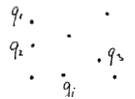
\includegraphics[width=\linewidth]{lecture_10/new_dipole1}
			\caption{Схематичное изображение диполя}
		\end{minipage}
		\begin{minipage}{0.68\linewidth}
			\begin{gather*}
				\dfrac{q_j q_k}{r_{jk}}, ~~
				j = 1, ~~ k = 2,\, 3, \dots; ~~~~ j = 2, ~~ k = 1,\, 3, \dots \\
				\Delta U = \dfrac{1}{2} \sum\limits_{j=1}^N \sum\limits_{k \neq j} \dfrac{q_j q_k}{r_{jk}}
			\end{gather*}
		\end{minipage}
	\end{figure}
	\begin{gather*}
		\Delta U = \dfrac { 1 } { 2 } N \sum\limits_{k=2}^N \dfrac{q_j q_k}{r_{jk}} \\
		\Delta G = \dfrac{1}{2}\, 2 N \left( -\dfrac{e^2 \kappa}{\eps} \right) \text{ (умножили на два, т.к. каждая частица считается дважды)} \\
		\kappa = \sqrt{ \dfrac{2 \pi e^2}{\eps kT} \sum n_{i, 0} Z_i^2 }
	\end{gather*}
	
	Введем понятие активности: $ a = \gamma C $, причем $ \gamma \rightarrow 1 $ при $ C \rightarrow 0 $. Рассмотрим химический потенциал:
	
	\begin{gather*}
		\mu_i = \underbrace{\mu_i^0 + RT \ln C_i}_{\text{идеал. раствор}} + RT \ln \gamma_i \\
		\ln \gamma_i = - \dfrac{Z_i^2 e^3}{(\eps kT)^{3/2}} \sqrt{ 2\pi \sum\limits_i C_i Z_i^2 } \\
		J = \dfrac{1}{2} \sum\limits_i C_i Z_i^2 \text{ --- ионная сила растовора} \\
		C \leq 0.01 \text{ H} \tab \ln \gamma_i = -Z_i^2 h \sqrt{J} \tab h = \text{const} \\
		C_+ = C_- = C \tab J = \frac{1}{2} (C \cdot 1^2 + C \cdot (-1)^2 ) = C \\
		\left.\begin{align*}
			&\Delta \phi = \kappa^2 \phi \\
			&1)~\phi = 0, ~ \dfrac{d \phi}{dr} = 0, ~~r \rightarrow \infty \\
			&2)~\phi|_{r=d} = \phi_0 \\
		\end{align*} \right\} \Rightarrow
		U = - \dfrac{e^2 \kappa}{\eps} \cdot \dfrac{1}{1 + \kappa d} \\
		\ln \gamma \sim \dfrac{ \sqrt{J} }{ 1 + \sqrt{J} } \tab J = 0.1
	\end{gather*}
%	Почему-то он создает лишнюю страницу, не будем делать этого
	\vspace*{-1cm}
\end{lecture}